%
%   Chapter Experiment
%
%   Qing-Cheng Li (r01922024 at csie dot ntu dot edu dot tw)
%   R.O.C.103.07
%
\chapter{實驗結果與分析}
\label{c:exp}

本章節進行了以樣式偵測特性的實驗,
以Wikipedia的文章作為模擬內容串流文件、
以YAGO的資料作為答案、
以PATTY提供的樣式對Wikipedia的文章進行偵測。
並介紹評估的標準以及對實驗結果的分析。

\section{測試資料集}
\label{s:dataset}

為了模擬內容串流文件,
本研究以Wikipedia的條目文章作為內容串流中的文件,
自2013年3月的Wikipedia Dumps\footnote{http://dumps.wikimedia.org/}擷取文件。

由於一開始並無文件中包含哪些實體特性的正確資料,
而YAGO的YAGO Facts提供了<subject, property, object>的資訊,
因此我們使用YAGO Facts的propety作為參考答案,
並將subject連結至Wikipedia的文章,
這樣就有每篇文件具有哪些特性的參考答案。

樣式則是使用PATTY提供的樣式釋義,其包含了知識庫定義的關係,
即本研究擬偵測之實體特性,以及可用以表達該特性之樣式集。
實驗採用的是其中的YAGO關係(YAGO Relations),一共有25組關係,
但其中一組關係(YAGO:Produced)在YAGO中沒有找到對映的Wikipedia條目,
因此僅對餘下24組關係進行實驗。

接下來只留下存在這24種特性的Wikipedia條目,
為了防止YAGO Facts中存在某特性但文章中卻根本沒有提及的狀況發生,
我們只留下<subject,property,object>中subject條目內有出現object字詞片段的特性留下,
若object內的字根本沒有出現在文章中,則捨去這個特性。
經過處理後,最後共有334,469篇條目作為測試資料集,
表\ref{t:yago-instance}顯示了各個特性在測試資料集中的數量。

%t:yago-instance
\begin{table}[t]
    \caption{各個特性於測試資料集中出現的文章數}
    \label{t:yago-instance}
    \begin{center}
        \small
        \begin{tabular}{|l|c|}
        \hline
        Property & Number of documents \\
        \hline
        actedIn & 3971\\
        created & 8665\\
        dealsWith & 111\\
        diedIn & 11729\\
        directed & 2036\\
        graduatedFrom & 10474\\
        happenedIn & 1792\\
        hasAcademicAdvisor & 628\\
        hasCapital & 363\\
        hasChild & 2113\\
        hasWonPrize & 8916\\
        holdsPoliticalPosition & 1190\\
        influences & 869\\
        isCitizenOf & 10974\\
        isKnownFor & 73\\
        isLeaderOf & 1397\\
        isLocatedIn & 216772\\
        isMarriedTo & 3555\\
        isPoliticianOf & 170\\
        livesIn & 7661\\
        participatedIn & 346\\
        playsFor & 42751\\
        wasBornIn & 47141\\
        worksAt & 1981\\
        \hline
        \end{tabular}
    \end{center}
\end{table}


表\ref{t:yago-coverage}統計了在不同的信心值下與不同的樣式歧義下,
樣式的數量以及含有這些樣式的文件總數。
由表中可以看出其實當樣式歧義度超過5之後所涵蓋的文件增長速度已經趨於平緩,
因此本實驗最多將只採用歧義度小於等於5的樣式進行。

%t:yago-coverage
\begin{table}[t]
    \begin{center}
        \small
        \begin{tabular}{|l||c|c|c|c||c|c|c|c|}
        \hline
        \multirow{2}{*}{歧義度} & \multicolumn{4}{ c|| }{信心值> 0} & \multicolumn{4}{ c| }{信心值> 0.7} \\
        \cline{2-9}
         & 樣式數 & 出現 & 涵蓋文章 & 比例
            & 樣式數 & 出現 & 涵蓋文章 & 比例 \\
        \hline
        1   & 11381 & 7267  & 250737    & 74.97 & 8913  & 5854  & 244888    & 73.22 \\
        2   & 4778  & 2976  & 275736    & 82.44 & 4175  & 2697  & 272395    & 81.44 \\
        3   & 1255  & 886   & 278820    & 83.36 & 1048  & 745   & 274265    & 82.00 \\
        4   & 666   & 503   & 281256    & 84.09 & 600   & 458   & 276782    & 82.75 \\
        5   & 635   & 465   & 283830    & 84.86 & 605   & 442   & 279603    & 83.60 \\
        \hline
        6   & 77    & 64    & 283858    & 84.87 & 68    & 57    & 279648    & 83.61 \\
        7   & 132   & 100   & 284128    & 84.95 & 131   & 100   & 280096    & 83.74 \\
        8   & 49    & 43    & 284275    & 84.99 & 49    & 43    & 280342    & 83.82 \\
        9   & 26    & 25    & 284295    & 85.00 & 26    & 25    & 280385    & 83.83 \\
        10  & 13    & 11    & 284297    & 85.00 & 13    & 11    & 280387    & 83.83 \\
        11  & 12    & 9 & 284299    & 85.00 & 12    & 9 & 280391    & 83.83 \\
        12  & 2 & 2 & 284299    & 85.00 & 2 & 2 & 280391    & 83.83 \\
        13  & 0 & 0 & 284299    & 85.00 & 0 & 0 & 280391    & 83.83 \\
        14  & 2 & 2 & 284299    & 85.00 & 2 & 2 & 280391    & 83.83 \\
        15  & 0 & 0 & 284299    & 85.00 & 0 & 0 & 280391    & 83.83 \\
        16  & 0 & 0 & 284299    & 85.00 & 0 & 0 & 280391    & 83.83 \\
        17  & 3 & 3 & 284299    & 85.00 & 3 & 3 & 280391    & 83.83 \\
        \hline
        總計 & 19031 & 12356    & -- & --   &15647 &10448 & -- & -- \\
        \hline
        \hline
        \multirow{2}{*}{歧義度} & \multicolumn{4}{ c|| }{信心值> 0.8} & \multicolumn{4}{ c| }{信心值> 0.9} \\
        \cline{2-9}
         & 樣式數 & 出現 & 涵蓋文章 & 比例
            & 樣式數 & 出現 & 涵蓋文章 & 比例 \\
        \hline
        1   & 5951  & 4029  & 222371    & 66.48 & 1879  & 1121  & 155402    & 46.46 \\
        2   & 2328  & 1697  & 251552    & 75.21 & 316   & 206   & 163265    & 48.81 \\
        3   & 683   & 487   & 258715    & 77.35 & 187   & 110   & 170820    & 51.07 \\
        4   & 473   & 355   & 261633    & 78.22 & 67    & 47    & 171978    & 51.42 \\
        5   & 278   & 243   & 262321    & 78.43 & 18    & 16    & 173397    & 51.84 \\
        \hline
        6   & 50    & 43    & 262364    & 78.44 & 10    & 8 & 173457    & 51.86 \\
        7   & 52    & 41    & 262452    & 78.47 & 12    & 8 & 174396    & 52.14 \\
        8   & 13    & 15    & 263419    & 78.76 & 2 & 2 & 174476    & 52.17 \\
        9   & 12    & 12    & 263514    & 78.79 & 8 & 8 & 175287    & 52.41 \\
        \hline
        總計    & 9840  & 6922  & --  & --  & 2499  & 1526  & --  & -- \\
        \hline
        \end{tabular}
        \caption{樣式總數量、出現數量、涵蓋文章與比例於不同信心值之統計}
        \label{t:yago-coverage}
    \end{center}
\end{table}


由於資料集內的Wikipeida條目皆是描寫實體,
在假設文章的內容都是以描寫該實體的前提下,
可以利用YAGO Simple Types作為該文描述實體之類型,
搭配樣式的領域(Domain)資訊輔助偵測。

而第\ref{c:method}章中所提到需要利用過去的資料進行統計、訓練分類器,
則是將測試資料集分為五等份,以其中四等份作為過去的資料,
並對其進行統計或訓練分類器,
餘下的一份進行測試。

\section{評估標準}
\label{s:eval}
在偵測系統的效率方面,
我們以每顆核心在每分鐘內可以處理多少文件來評估,
以及要達到TREC知識庫加速競賽的每小時處理約100,000篇的規模需要多少運算核心或機器。

在偵測系統的效能方面,
我們希望了解對每一個實體特性,
利用樣式自文章中偵測該特性的效能。
因此,以精確率(Precision)、召回率(Recall)、$F_1$分數($F_1$ Score)進行評估。
精確率公式如式\ref{f:precision},召回率公式如式\ref{f:recall}。

\begin{equation}
    \label{f:precision}
    Precision = \frac{|\{relevant\ documents\}\cap\{retrived\ documents\}|}{|\{retrived\ documents\}|}
\end{equation}

\begin{equation}
    \label{f:recall}
    Recall = \frac{|\{relevant\ documents\}\cap\{retrived\ documents\}|}{|\{relevant\ documents\}|}
\end{equation}

對於一個實體特性,經過偵測之後會有被標為有此特性的文件與無此特性的文件。
其中,相關的文件(Relevant documents)即真正存在該特性之文件;
尋回的文件(Retrived documents)即偵測系統標記為擁有此特性之文件。
精確率評估在尋回的文件之中有多少文件真正存在該特性;
召回率評估在真正擁有該特性的文件中有多少被系統偵測到。

$F_1$分數則是綜合評估精確率與召回率,計算方式如式\ref{f:f1},為精確率與召回率的調和平均。

\begin{equation}
    \label{f:f1}
    F_1\ Score = \frac{2\times Precision \times Recall}{Precision + Recall}
\end{equation}

除了評估個別特性的效能之外,以宏觀平均(Macro Average)及微觀平均(Mirco Average)分別計算精確率與召回率及$F_1$分數來評估整體效能。
以精確率為例,宏觀平均的計算如式\ref{f:macro},
而微觀平均的計算則如式\ref{f:micro}。

\begin{equation}
    \label{f:macro}
    Macro\ Avg\ Precision=\frac{\sum_i^n precision_i}{n}
\end{equation}

\begin{equation}
    \label{f:micro}
    Mirco\ Avg\ Precision=\frac{\sum_i^n |\{relevant\ documents\}_i|\cap|\{retrived\ documents\}_i|}{\sum_i^n |\{retrived\ documents\}_i|}
\end{equation}

\section{實驗結果}
\label{s:result}

\subsection{效率}
在圖\ref{i:process-v2}的偵測流程之中,本實驗將其拆解為兩個部份來評估效能。
前半部份為樣式比對的效率,後半部份為特性消歧義的效率。

樣式比對的效率在時脈為2.5GHz的中央處理器為每顆核心每分鐘592份文件,
特性消歧義的效率在同樣條件下為每顆核心每分鐘2750份文件。
要在一小時內處理100,000文件僅需要3顆核心即可完成。
而本實驗使用一台配備時脈2.5GHz、24核心中央處理器的工作站僅需半小時即可處理完全部約330,000份文件。

\subsection{原始效能}
依照圖\ref{i:process-v2}的流程,
但於樣式篩選的部分僅篩選了無歧義度以及歧義度小於等於5的樣式,
而無特性消歧義的結果如表\ref{t:baseline-1}。
表中左半部是每一個特性使用無歧義度,也就是歧義度為1的樣式,
進行特性偵測的結果,由於沒有歧義問題,所以無需進行特性消歧義。

右半部則使用了歧義度5及更小的樣式,而不進行特性消歧義,
可以看到的結果是,由於沒有進行特性消歧義而的對每篇文章回答盡可能多的特性,
因此召回率提升,但精確率也因此下降,$F_1$分數則因為精確率降太多而變低。

由此也可以看出太寬鬆地依據樣式回報特性會降低效能,
後續的實驗將陸續加入樣式篩選與特性消歧義的方法, 嘗試改善效能。

%t:baseline-1
%\begin{sidewaystable}
\begin{table}
    \begin{center}
        \scriptsize
        \begin{tabular}{|l||c|c|c||c|c|c|}
        \hline
        \multirow{2}{*}{Property} & \multicolumn{3}{ c|| }{歧義度1} & \multicolumn{3}{ c| }{歧義度5無篩選} \\
        \cline{2-7}
        & Precision & Recall & $F_1$ Score & Precision & Recall & $F_1$ Score \\ 
        \hline
        actedIn & 0.04346684 & 0.51633265 & 0.0801835267 & 0.02808748 & 0.7975619 & 0.0542639635\\
        created & 0.08228679 & 0.81709385 & 0.1495162939 & 0.05583113 & 0.95001754 & 0.1054642798\\
        dealsWith & 0.00335447 & 1 & 0.0066865103 & 0.00216425 & 1 & 0.0043191523\\
        diedIn & 0.06224856 & 0.36879393 & 0.1065179958 & 0.05507079 & 0.64684916 & 0.1015001618\\
        directed & 0.03927418 & 0.28666455 & 0.0690836289 & 0.02895369 & 0.94029186 & 0.0561775476\\
        graduatedFrom & 0.14718304 & 0.47521937 & 0.2247556578 & 0.11298864 & 0.78572966 & 0.19756697\\
        happenedIn & 0.13234375 & 0.66757981 & 0.2208961453 & 0.13154836 & 0.67313236 & 0.2200859442\\
        hasAcademicAdvisor & 0.02812044 & 0.43292079 & 0.0528105614 & 0.01292023 & 0.68924446 & 0.0253649808\\
        hasCapital & 0.05295147 & 0.34298641 & 0.0917398184 & 0.00585946 & 0.45816088 & 0.0115709382\\
        hasChild & 0.02842344 & 0.63019974 & 0.0543936048 & 0.01822775 & 0.97241921 & 0.0357847245\\
        hasWonPrize & 0.12120602 & 0.01099484 & 0.0201608491 & 0.09693382 & 0.07378178 & 0.0837878879\\
        holdsPoliticalPosition & 0.03016289 & 0.75982481 & 0.0580224532 & 0.01514724 & 0.89445116 & 0.0297899961\\
        influences & 0.0153143 & 0.82712489 & 0.0300718173 & 0.00816085 & 0.9559357 & 0.0161835407\\
        isCitizenOf & 0.11992498 & 0.12948061 & 0.1245197396 & 0.08785729 & 0.39014472 & 0.1434180488\\
        isKnownFor & 0.00212329 & 0.44639731 & 0.0042264768 & 0.00079513 & 0.93804714 & 0.0015889132\\
        isLeaderOf & 0.04677461 & 0.02328296 & 0.0310901841 & 0.01930836 & 0.469555 & 0.0370914972\\
        isLocatedIn & 0.84517473 & 0.52077778 & 0.6444561087 & 0.77085313 & 0.56178423 & 0.6499189428\\
        isMarriedTo & 0.03827487 & 0.6623392 & 0.0723677924 & 0.02744828 & 0.96646594 & 0.0533805175\\
        isPoliticianOf & 0.01632025 & 0.23554096 & 0.0305254418 & 0.00369108 & 0.7024813 & 0.0073435743\\
        livesIn & 0.07468026 & 0.05527752 & 0.0635304722 & 0.06734495 & 0.44379567 & 0.116943933\\
        participatedIn & 0.02227683 & 0.65485327 & 0.043087894 & 0.02020859 & 0.71510601 & 0.039306398\\
        playsFor & 0.52387168 & 0.51813046 & 0.5209852535 & 0.38285718 & 0.6095533 & 0.4703131662\\
        wasBornIn & 0.28617774 & 0.082453 & 0.1280208655 & 0.25226525 & 0.39620268 & 0.3082594019\\
        worksAt & 0.04388619 & 0.35625107 & 0.078145695 & 0.02095881 & 0.86501083 & 0.040926002\\
        \hline
        Macro Average & 0.11690923 & 0.45085499 & 0.1856725305 & 0.09272841 & 0.70398844 & 0.1638718415\\
        Micro Average & 0.22569929 & 0.4356432 & 0.297347781 & 0.12550728 & 0.56034827 & 0.205080464\\
        \hline
        \end{tabular}
        \caption{僅使用無歧義的樣式與歧義度5篩選之實驗結果}
        \label{t:baseline-1}
    \end{center}
%\end{sidewaystable}
\end{table}


\subsection{樣式篩選}
\subsubsection{信心值}
我們利用PATTY提供的信心值進行樣式的篩選,選定了門檻值分別為0(沒有門檻)、0.7、0.8與0.9,
只使用樣式信心值大於門檻值的樣式進行偵測實驗,其結果的宏觀平均與微觀平均$F_1$分數如圖\ref{i:conf-f1}所示。

\begin{figure}
    \centering
    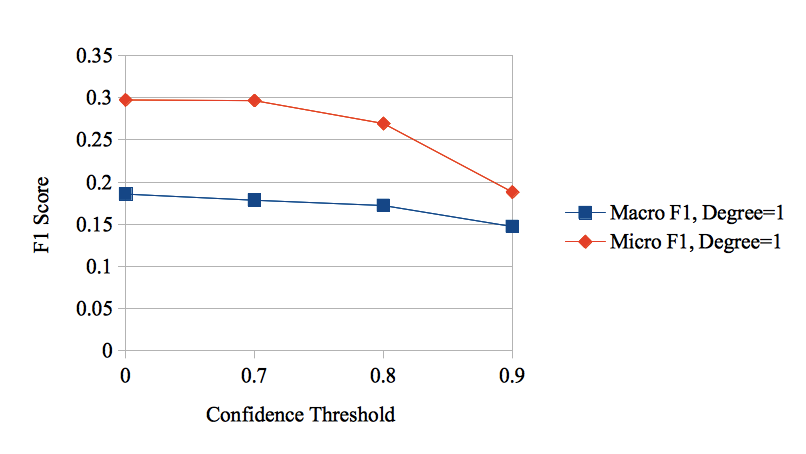
\includegraphics[width=0.85\textwidth]{images/04-conf-f1}
    \caption{無歧義度下F1分數平均隨信心值變化圖}
    \label{i:conf-f1}
\end{figure}

就整體效能而言,設定信心值門檻值並沒有辦法提升系統效能,反而使效能變差。
這是由於設定門檻值後,通過門檻值的樣式數量減少,導致召回率下降太多,
到門檻值為0.9時,有部分的特性(hasCapital, isKnownFor)已經沒有可用的樣式。
但部分的特性$F_1$分數因精確率比較大幅度的提升而略微上昇,表\ref{}中,
特性%TODO: list those property
的精確率皆有比較大幅度的提升。

% TODO
% build table

\subsubsection{可信賴度}


\subsubsection{歧義度}

\subsection{特性消歧義}
\subsubsection{實體類型資訊}
\subsubsection{正規化?}
\subsubsection{簡單貝氏分類器}
%\subsecion{}
%錯誤分析
